\documentclass{acm_proc_article-sp}
\makeatletter
\def\@copyrightspace{\relax}
\makeatother

\usepackage{graphicx}
\usepackage{url}
\usepackage{eurosym}

\begin{document}

% 1. Report title, authors, and support cast (Lab assistant and course instructors). For each person, give name and contact information (email).
\title{GaussianCloud}
\subtitle{A Cloud-Based Image Blurring Application}

\numberofauthors{5}
\author{
\alignauthor
R.M. de Lange\\
		\affaddr{1534068}\\
		\email{\{r.m.delange,}
\alignauthor
M. Voinea\\
		\affaddr{4317602}\\
		\email{m.voinea\}@student.tudelft.nl}
\and
\alignauthor
D.H.J. Epema\\
		\affaddr{Course Instructor}\\
		\email{\{d.h.j.epema,}
\alignauthor
A. Iosup\\
		\affaddr{Course Instructor}\\
		\email{a.iosup,}
\alignauthor
B.I. Ghit\\
		\affaddr{Lab Assistant}\\
		\email{b.i.ghit\}@tudelft.nl}
}

\maketitle

% 2. Abstract: a description of the problem, system description, analysis overview, and one main result. Size: one paragraph with at most 150 words.
\begin{abstract}
This report analyses the opportunity for WantCloud to apply an IaaS system to process their image blurring workload.
WantCloud has irregular loads on their current system and wants an efficient way to deal with this, giving optimal speed and keeping costs low.
Furthermore, WantCloud wants to improve the reliability of the system by eliminating the single point of failure.
The proposed system uses the Amazon Compute Cloud to host a number of machines that perform the tasks.
These Worker nodes are directed by a Master node, which assigns the tasks through a Scheduler.
A Backup node ensures reliability by monitoring the Master and taking over if necessary.
To verify the usability, the processing times, overhead and recovery times of the proposed system were analysed.
From this it followed that the system offers flexibility, reliability and faster image processing, whilst minimising overhead and costs.
\end{abstract}

% 3. Introduction (recommended size, including points 1 and 2: 1 page): describe the
% problem, the existing systems and/or tools (related work), the system you are about to
% implement, and the structure of the remainder of the article; use one short paragraph
% for each.
\section{Introduction}
\label{sec:intro}
WantCloud BV is a multi-faceted organisation which has recently started a development branch in the image processing domain.
The most expensive operation required by WantCloud's new business processes involves applying a Gaussian blur to images.
This process is compute intensive, as Gaussian functions require complex calculations as well as reading and writing large amounts of data.
Moreover, it scales non-linearly with the size of the uploaded images.

Currently, WantCloud has a single server running all of these tasks.
For applying the Gaussian blur, an image filtering implementation in Java by Jerry Huxtable is used.\cite{web:huxtable}
The WantCloud server is experiencing heavy peak loads and sits idle for the rest of the day.
At peak moments, clients need to wait for quite some time for the images to be processed, which is harmful for WantCloud's business.
Therefore, WantCloud wants to explore the option to utilise a cloud computing infrastructure to cope with high loads and be able to scale down with low loads.

This report will discuss the details of an exploration towards using Amazon EC2\cite{web:ec2} as a solution to WantClouds needs.
The image processing system will be implemented on a dynamically scalable cluster of compute nodes.
This implementation is made available open source through GitHub\cite{web:git}.
The performance, overhead, and scalability will be tested to compare to the current set-up using one machine.

In this report, insight will first be given into the background of the application and its requirements in Section \ref{sec:bg}.
After this, the design of the cloud solution will be discussed in Section \ref{sec:system}, giving an overview of the implementation.
The designed system will be tested and evaluated in Section \ref{sec:eval}.
The results of the evaluation will be discussed in Section \ref{sec:discussion} and conclusions will be presented in Section \ref{sec:conclusion}.

% 4. Background on Application (recommended size: 0.5 pages):
% describe the application (1 paragraph) and its requirements (1-3 paragraphs, summarized in a table if needed).
\section{Background}
\label{sec:bg}
The application that WantCloud uses receives images of varying sizes, to which a Gaussian blur needs to be applied.
As the image files are uploaded, they are processed by the WantCloud server, and the results are stored to be presented to the clients, or further processed through other manipulations.
Currently, WantCloud uses a single machine to process these images.
This machine has to process many image files at certain times and sits idle for most of the time.

WantCloud has decided to explore the option of using a cloud platform to handle these varying loads in a more efficient way.
This means that the explored solution should provide better performance, while keeping the resulting costs to a minimum.
More specifically, the application has to deal with the following requirements.

\subsection{Elasticity}
The application must automatically provision compute nodes, depending on the current workload.
This means that unused nodes should be released as they are no longer needed, and new nodes should be leased as soon as the workload increases.
No human input should be required to carry out the process.
This requirement should result in being able to handle peak loads better, while limiting costs for unused resources.

\subsection{Load Balancing}
The application should automatically schedule tasks to compute nodes.
This means that tasks are divided over available nodes, new nodes are started when needed, and unused nodes are released without human input.

\subsection{Reliability}
Furthermore, the application must be reliable, or fault tolerant.
This means that any problems that occur should be dealt with, without the need for human interference.
Nodes that crash, tasks that break or other problems that occur should be dealt with by the system automatically.

\subsubsection{Monitoring}
Although WantCloud wishes to create a system that performs without human intervention, it does want to be able to monitor the work.
Specifically, it wants to monitor which tasks have been processed, by what machine the task was processed, and how long each machine has been active.
This is important for both billing and testing purposes.

% 5. System Design (recommended size: 1.5 pages)
% c. (Optional, for bonus points, see Section F) Additional System Features:
% describe each additional feature of your system, one sub-section per feature.
\section{System Design}
\label{sec:system}
The system was designed with efficiency in mind.
WantCloud wants to be able to run the system as they do now, without them having to actively monitor and provision machines.
With this in mind, the main design decisions were made to comply with the requirements discussed in Section \ref{sec:bg}.
In this section, the main aspects of the system design will be discussed: the architecture, resource management, policies, and actual implementation.

\subsection{Architecture Overview}
The architecture of this solution is kept simple, it consists of Master and Worker nodes.
These nodes communicate to notify each other of new tasks and finished tasks.
Figure \ref{fig:architecture_overview} gives an overview of the discussed architecture.
A short description of all elements in the overview follows.

\begin{figure}
	\centering
	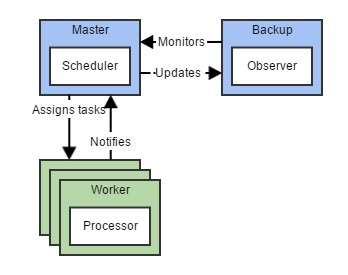
\includegraphics[width=0.4\textwidth]{images/architecture_overview.jpg}
	\caption{An overview of the system architecture on a high level. Multiple Workers are controlled by a Master node. The Backup node monitors the state of the Master node.}
	\label{fig:architecture_overview}
\end{figure}

\subsubsection{Master and Scheduler}
The Master node is the heart of the system, it receives new tasks and handles the scheduling.
The Master keeps a queue of all tasks that still need to be performed.
It assigns these tasks to Worker nodes and gets notified of finished tasks by the Workers.
The assignment of tasks is done by the Scheduler.
Furthermore, the Scheduler instantiates new Worker nodes when the queue becomes too long.
These Worker nodes are stopped again when they have been inactive for a set period of time.
The scheduling policy will be further addressed in Section \ref{sec:policies}.

\subsubsection{Backup}
The Backup node monitors the state of the Master node and receives updates on new and finished tasks.
Incoming and processed images are also sent to the Backup node, so that they are available when the Master goes down.
The Backup node takes over the Masters work when the Master node becomes unavailable.

\subsubsection{Worker}
Worker nodes perform the actual work, they blur the image by applying a Gaussian filter.
These nodes receive tasks from the Master node, process them, and reply to the Master whenever a task is finished.
Worker nodes do not manage their own queue, they process one task at a time.


% a. Resource Management Architecture: describe the design of your system,
% including the inter-operation of the provisioning, allocation, reliability, and
% monitoring components (which correspond to the homonym features required
% by the WantCloud CTO).
\subsection{Resource Management Architecture}
\label{sec:resource_man}
This section will discuss how the designed architecture manages the resources of the cloud infrastructure.
Management of these resources is done according to the requirements given in Section \ref{sec:bg}.

\subsubsection{Elasticity}
The Scheduler, as discussed previously, manages the provisioning of Worker nodes as needed.
As the workload increases, the queue in the Master node builds up.
At a predetermined queue length, new Worker nodes will be provisioned.
These nodes are monitored by the Scheduler and stopped after a set period of inactivity.
The exact provisioning policy will be discussed in Section \ref{sec:policies}.

\subsubsection{Load Balancing}
The Scheduler balances the load by assigning tasks to the first available Worker node.
It does so by keeping track of all nodes and their states.
The four states a Worker node can be in are: Stopped, Starting, Idle, and Working.
As the names suggest, they imply that the node is turned off, starting up, waiting for work or processing a task respectively.
An Idle node is ready to receive a new task, it is therefore preferred as a node to assign tasks to.
If no Idle node can be found, the Scheduler either waits for a node to become Idle or provisions a new one, depending on the length of the queue.

\subsubsection{Reliability}
To ensure reliability, two monitoring features have been built into the design.
Dectection and recovery from failure of a Worker node is handled by the Master, who monitors the Workers.
If a Worker node does not finish a tasks within a given period of time, it is assumed that the node crashed and it is shut down.
The task that Worker was working on will then be reintroduced to the queue and assigned to the next available node.

The second monitoring feature is the Backup node, responsible for handling Master node failures.
This node receives all uploaded/processed images from the Master as well as all incoming connections from Worker nodes.
If no message can be sent, the Master notifies the Backup that it is still alive.
This way the Backup node knows if the Master is still working properly.
When there is no communication for a given period of time, the Backup node takes over and notifies all Workers that it has become the Master node.
Furthermore, the Master node is rebooted and initiated as a new Backup node.

Failure of the Backup node is also handled in the Master, but not through a monitoring solution.
A sudden break down of the Backup's functionality will cause the Master's outgoing buffer of messages to the Backup to overflow, thus closing the connection. Once the Master senses the connection is lost, it reboots the Backup and registers all past and current image file traffic to be re-replicated to the new Backup once it connects.

\subsubsection{Monitoring}
To monitor all the work that is being done in the system, logs are kept.
These logs are written to files on each server, keeping track of its own work.
The Master node logs the assignment and completion of tasks.
Worker nodes log incoming tasks, their processing and their completion.
These logs give an insight in processing times and load on each node.

% b. System Policies: describe the policies your system uses and supports. The latter
% may remain not implemented throughout your coursework, as long as you can
% explain how they can be supported in the future.
\subsection{System Policies}
\label{sec:policies}
As mentioned in several previous sections, specific functions of the system are controlled through policies.
Especially the work of the Scheduler depends very much on these set policies.
The following subsections will discuss the use of these policies, their current settings, and the possibility to extend this using custom policies.

\subsubsection{Scheduling}
Scheduling, consisting of load balancing and provisioning, is the core of the designed system.
It is used to assign tasks to available nodes, making optimal use of resources.
The Scheduler component has several settings that help it perform best, mostly related to the provisioning of new nodes.
The system stores these settings in a properties file, they are summed up in Table \ref{tbl:policy}.

\begin{table}
	\centering
	\begin{tabular}{| l | l | r |}
		\hline
		Setting name & Description & Value \\ \hline \hline
		\texttt{interval} & Scheduler interval & 2 sec. \\ \hline
		\texttt{loadThresh} & Max. tasks in queue & 5/node \\ \hline
		\texttt{maxTaskTime} & Max. time a Worker is Working & 1 min. \\ \hline
		\texttt{maxIdleTime} & Max. time a Worker is Idle & 1 hour \\ \hline
		\texttt{maxTaskRetry} & Max. times a task is retried & 2 x\\ \hline
		\texttt{maxTimeOut} & Max. times Master is unresponsive & 10 sec. \\ \hline
	\end{tabular}
	\caption{Settings for the different policies. These values describe the behaviour of the scheduling and the reliability policies.}
	\label{tbl:policy}
\end{table}

The basic choice for the scheduler is to assign a new task to the first available Worker node.
When no Worker node is available the Scheduler checks the length of the queue with the given policy.
As seen in Table \ref{tbl:policy}, the value of \texttt{loadThresh} indicates that if more than 5 tasks per working node are in the queue, a new Worker node should be provisioned.
This number was chosen as processing 5 tasks generally takes longer than provisioning a new Worker.

When a Worker node has been Idle for an hour, as set by \texttt{maxIdleTime}, it is shut down.
This period was chosen because the system is run on the Amazon EC2 cloud, in which starting up a machine costs the equivalent of one hour of compute power.
Shutting down a machine sooner and provisioning it again multiple times within an hour would cause a tremendous increase in cost.

\subsubsection{Reliability}
The other settings in Table \ref{tbl:policy} are used for reliability of the system.
\texttt{maxTaskTime} is used to indicate after what period the Master can consider a Worker node to have crashed, in this case it is set to 1 minute.
However, it should be considered that this period should be substantially longer than the maximum length an actual (non-crashed) task might take.

\texttt{maxTaskRetry} is the maximum amount of times a task is reassigned after a Worker node crashed on it.
With these settings if two nodes fail on the same task, the task is considered corrupt and ignored for further processing.

\texttt{maxTimeOut} is the maximum period in which the Backup node has not been able to contact the Master node.
If this period has passed, the Backup node takes over as the Master node.
This period is set to 10 seconds, as the Master node should normally send a message to the Backup node every 2 seconds (the \texttt{interval} setting).

\subsubsection{Extensions}
As the implemented policies are stored in properties files, they can easily be replaced or edited.
This allows the designed system to support different policies as well as enables WantCloud to fine-tune the policies according to the monitoring results.
Flexibility added this way allows the system to be adapted to changes in the environment, or nature of the tasks it performs.

\subsection{Implementation}
The system is implemented in approximately 3500 lines of Java. 
It consists of a single Maven\cite{web:maven} project that packages itself as a Java archive (jar). 
The jar can be run to start up either a Master, a Backup or a Worker instance by altering the command line options.

\subsubsection{Node Instance}
The Master, the Backup and all Workers are extensions of a node instance.  
Each node has basic communication abilities and awareness of its physical node identifier, which it uses as a signature in communication. 

\subsubsection{Derived Instances}
The derived instances implement the necessary processing functionality, resource management and policies described earlier in this section.
Regular and long-running application logic runs as a separate thread. 
For instance, the Master's Scheduler, the Backup's MasterObserver, and the Worker's Processor are all threads that carry out their specific functionality. 
The take-over procedure is implemented as a forced instantiation of a new Master instance by the Backup, followed by a forced stopping of all threads carrying out Backup functionality.

\subsubsection{Communication}
Communication between the nodes is done via the Java NIO API\cite{web:nio} specification, using the server-client pattern. 
Each node instance keeps a running Server thread that listens for new connections, and a set of Client threads for each node that it connects to.
 The master is only connected \emph{to} and does not keep any clients. 
Workers connect only to the master, but keep a Server to listen for take-over messages from the backup instance. 
The backup instance only keeps clients to connect to the master and each worker that it is notified of by the master. 
The communication consists of serialized Message objects that are sent and received over non-blocking sockets, in order to avoid communicators getting \lq{}stuck\rq{} on transfer operations. 
These messages have an identifier, an owner (the emitting node's signature), a data object (the image file's content as a byte array, if applicable) and details (such as the image identifier). 
Since image files are large in size, the message bytes are grouped into segments before they are sent.

% 6. Experimental Results (recommended size: 1.5 pages)
% a. Experimental set-up: describe the working environments (DAS, Amazon EC2,
% etc.), the general workload and monitoring tools and libraries, other tools and
% libraries you have used to implement and deploy your system, other tools and
% libraries used to conduct your experiments.
\section{Evaluation}
\label{sec:eval}
To verify whether the designed system offers an improvement to WantCloud, experiments have been conducted.
These experiments analyse the performance of the system as well as analyse the previously described features.
This section will first discuss the experimental set-up, giving an overview of the used environment and the implementation of the proof of concept.
Following subsections will discuss the conducted experiments and their results.

\subsection{Experimental Set-up}
The working environment chosen for this system is Amazon Web Services\cite{web:aws}, particularly the Elastic Compute Cloud (EC2)\cite{web:ec2}.
Virtual machines called EC2 instances can easily be provisioned on this infrastructure.
Moreover, the platform offers many tools to create divers applications.

The chosen instances are \texttt{t2.micro} instances with an Ubuntu operating system.
This instance type only offer one virtual CPU and 1 gigabyte of memory.
However, these instances can be used free of charge for 750 hours per month, leaving enough space to perform the experiments at no cost.
Six of these instances were created, of which one functioned as Master node, one as Backup node and four as Worker nodes.

The implementation of the system was done in Java and applies several external tools to perform all its work.
The most notably are the Gaussian blur implementation by Huxtable \cite{web:huxtable} and the AWS SDK for Java \cite{web:sdk}, used for starting and stopping instances.
The full implementation of the experimental set-up is available as open source through GitHub \cite{web:git}.

% b. Experiments: describe the experiments you have conducted to analyse each
% system feature, then analyse them; use one sub-section per experiment. For
% each experiment, describe the workload, present the operation of the system,
% and analyse the results. In the analysis, report:
% i. Charged-time = time that would have been charged using the
% Amazon EC2 timing approach (1-hour increments)
% ii. Charged-cost = cost that would have been charged using the
% Amazon EC2 charging approach, assuming 10 Euro-cents/charged hour
% iii. Service metrics of the experiment, such as runtime and response time of
% the service, etc.
% iv. (optional) Usage metrics of the experiment, such as per-VM and overall
% system usage and activity.
\subsection{Scheduler Performance}
The first conducted experiment tests the performance of several scheduler set-ups against the performance of the current WantCloud server.

\subsubsection{Test Set}
To understand this experiment, it is important to first describe the test set that was used.
The total test set consists of 20 images, which are listed in Table \ref{tbl:tasks}.
The table shows the file name, their size in kilobytes, their occurrence in the test set (\#), and the average time it took to process that image over all tests.
This set consists of four different images, of different sizes representing typical images.
There are two occurrences of the rather large \emph{strawberry.jpg}, and more occurrences of the smaller images.
As can be expected, it is easier to compute a Gaussian filter for small images than it is for large images.

\begin{table}
	\centering
	\begin{tabular}{| l | r | c | r |}
		\hline
		File name & Size (kB) & \# & Avg. time (sec.) \\ \hline \hline
		\emph{apple.jpeg} & 90.5 & 4 & 0.548 \\ \hline
		\emph{banana.jpg} & 342.2 & 7 & 17.312 \\ \hline
		\emph{pears.jpg} & 957.2 & 7 & 17.468 \\ \hline
		\emph{strawberry.jpg} & 5,735.9 & 2 & 26.226 \\ \hline
	\end{tabular}
	\caption{Selected set of test images, their size in kilobytes, their occurrence in the test set (total: 20 images), and their average processing time over all tests.}
	\label{tbl:tasks}
\end{table}

\subsubsection{Experiment}
In this experiment the current WantCloud approach is simulated by using a single EC2 instance that operates directly on input files, without the use of a scheduler.
The used set-ups are listed in Table \ref{tbl:setups}.
In this table, the \emph{Single} set-up is the instance just described.
The other set-ups use the Scheduler and have respectively one, two, three or four Worker nodes to perform the work. 

\begin{table}
	\centering
	\begin{tabular}{| l | c | c |}
		\hline
		Name & Scheduler & \# Worker \\ \hline \hline
		\emph{Single} & no & - \\ \hline
		\emph{Scheduler 1} & yes & 1 \\ \hline
		\emph{Scheduler 2} & yes & 2 \\ \hline
		\emph{Scheduler 3} & yes & 3 \\ \hline
		\emph{Scheduler 4} & yes & 4 \\ \hline
	\end{tabular}
	\caption{The different set-ups tested in the Scheduler Performance experiment, the name, use of the Scheduler, and amount of used Worker nodes are listed.}
	\label{tbl:setups}
\end{table}

\begin{figure}
	\centering
	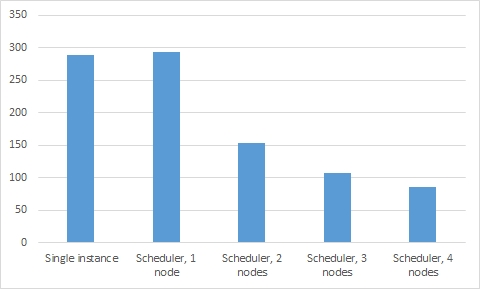
\includegraphics[width=0.5\textwidth]{images/diagram_total_processing.jpg}
	\caption{Processing time comparison for 5 types of set-ups. Time in seconds.}
	\label{fig:diagram_total_processing}
\end{figure}

\newpage

\subsubsection{Results}

The results of this experiment are shown in Figure \ref{fig:diagram_total_processing}.
This figure shows the total processing time for the whole test set per set-up.
Several interesting facts stand out when analysing these results.
First of all it can be seen that \emph{Scheduler 1} takes a few seconds longer than \emph{Single}.
This is as expected, as the Scheduler would cause some overhead.
Interestingly, this overhead is quite minimal.
The following observation that can be made is that \emph{Scheduler 2} scores significantly better than both previous set-ups.
The speed up is almost double compared to \emph{Scheduler 1}.
\emph{Scheduler 3} and \emph{Scheduler 4} both perform even better than the previous two.

To verify these results the average processing time per task was also analysed in Figure \ref{fig:diagram_avg_image}.
This figure shows that the average time per task is almost the same in each set-up.
A small increase can be seen from \emph{Single} to the \emph{Scheduler} set-ups, which could be due to the Scheduler overhead.
However, this difference is so small it is hardly measurable on this scale.

Table \ref{tbl:costs} gives an overview of estimated costs using the different set-ups on Amazon EC2.
For \emph{Single} only one machine is needed, which keeps the cost low.
For \emph{Scheduler 1} to \emph{4}, not only the Worker node, but also a Master node and a Backup node are required, this results in higher costs per running hour.
As these tests were relatively brief, they do not predict the costs for long term use of the system.
In the long term, the \emph{Scheduler} set-ups require at least two machines to be running at all time (Master and Backup), Workers can be shut off.
Further discussion of these costs can be found in Section \ref{sec:discussion}.

\begin{table}
	\centering
	\begin{tabular}{| l | c | c |}
		\hline
		Name & EC2 hours & Costs (\euro) \\ \hline \hline
		\emph{Single} & 1 & 0,10 \\ \hline
		\emph{Scheduler 1} & 3 & 0,30 \\ \hline
		\emph{Scheduler 2} & 4 & 0,40 \\ \hline
		\emph{Scheduler 3} & 5 & 0,50 \\ \hline
		\emph{Scheduler 4} & 6 & 0,60 \\ \hline
	\end{tabular}
	\caption{The charged hours and costs of the different set-ups tested in the Scheduler Performance experiment, on Amazon EC2. Cost per hour: \EUR{0,10}.}
	\label{tbl:costs}
\end{table}

\begin{figure}
	\centering
	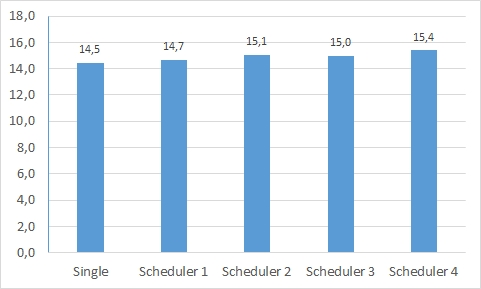
\includegraphics[width=0.5\textwidth]{images/diagram_avg_image.jpg}
	\caption{Average processing time per task for 5 types of set-ups. Time in seconds.}
	\label{fig:diagram_avg_image}
\end{figure}

\subsection{Time To Recover Master}
The most expensive recovery procedure is that from a Master failure. 
A series of experiments were conducted to measure the time it takes for the new Master to restart processing, as well as what overhead this redundancy incurs on the processing time.

\subsubsection{Time Experiment}
The first experiment type was intended to measure recovery time. 
The maxTimeOut setting was fixed at 5 seconds. 
The Master, Backup and Worker instances were started and normal processing began on the same test set as before. 
However, after an arbitrary time, the Master was purposely shut down, leaving the Backup to take over. 

\subsubsection{Time Results}
The Backup took over processing tasks at an average of 20 seconds after it lost connection to the master.
This means that it took 15 seconds for the Backup to start up a new Master instance, notify all Workers to connect to it, recover all the previous Master's connections and start processing once more.

\subsubsection{Overhead Experiment}
The second type of experiment was meant to measure how much overhead replication to the Backup actually incurs. 
The same test set was used with the 4 scheduler configurations as before. 
Processing was run once without connecting a Backup node to the Master, and again with the Backup node receiving replicated data from the Master.

\subsubsection{Overhead Results}
Table \ref{tbl:overhead} shows the extra time needed for the replication to be done in each of the 4 configurations. 
The average is 5,1 seconds, which is negligible compared to the duration of the processing. 
It is interesting to see that the added overhead does not depend on the configuration. 
We argue that the large variability is due to the fluctuation in network availability and computation power in the virtual machines on which the Master and Backup processes run.

\begin{table}
	\centering
	\begin{tabular}{| l | r |}
		\hline
		Name & Extra time (sec.) \\ \hline \hline
		\emph{Scheduler 1} & 3,6 \\ \hline
		\emph{Scheduler 2} & 12,7 \\ \hline
		\emph{Scheduler 3} & 3,2 \\ \hline
		\emph{Scheduler 4} & 0,9 \\ \hline \hline
		Average & 5,1 \\ \hline
	\end{tabular}
	\caption{The extra time it takes for processing to end in the different configurations, when a Backup node receives replicas of the input/processed files.}
	\label{tbl:overhead}
\end{table}

\subsection{Time To Boot}
To be able to fully use the provisioning capabilities of the designed system, it is important to know the time it takes for a Worker to be instantiated.
This time period is relevant for the Scheduler to be able to assess whether or not the queue is long enough to initialise more Worker nodes.
The relevant time is measured from the moment the Master node sends a request to start an instance to the AWS API, until the Worker node connects to the Master.
At that moment the Worker node is ready to accept tasks.

\subsubsection{Experiment}
For this experiment, the existing implementation was used, with a small addition.
To measure only the time it takes to start an instance as well as run the Worker software on it, a specific command was added to the Master implementation.
This command allows to start the process of booting up a new Worker, as would normally happen through the Scheduler, but without the processing of tasks.

\subsubsection{Results}
All four Worker instances were started up and the time it took for them to connect was recorded.
The results found in this experiment are listed in Table \ref{tbl:boottimes}.
On average it takes a Worker 32,3 seconds to be ready to process tasks.
As seen in Figure \ref{fig:diagram_avg_image}, a single task takes roughly 15 seconds. 
From this we can deduct that already at 4 tasks per working node, it might be useful to start a new Worker.
The current policy is set to 5, which is a more safe choice.

\begin{table}
	\centering
	\begin{tabular}{| l | r |}
		\hline
		Machine & Boot time (sec.) \\ \hline \hline
		\emph{Worker 1} & 30,7 \\ \hline
		\emph{Worker 2} & 26,7 \\ \hline
		\emph{Worker 3} & 30,7 \\ \hline
		\emph{Worker 4} & 41,4 \\ \hline \hline
		Average & 32,3 \\ \hline
	\end{tabular}
	\caption{The time it takes from the moment the Master sends a command to boot up until the Worker connects to the Master and is ready to receive tasks.}
	\label{tbl:boottimes}
\end{table}


% 7. Discussion (recommended size: 1 page): summarize the main findings of your work
% and discuss the tradeoffs inherent in the design of cloud-computing-based applications.
% Should the WantCloud CTO use IaaS-based clouds? Among others, use extrapolation
% on the results, as reported in Section 6.b of the report, to discuss the charged time and
% charged cost reported in section for 100,000/1,000,000/10,000,000 users and for 1
% day/1 month/1 year.
\section{Discussion}
\label{sec:discussion}
% TODO: discuss costs in long term use of this cloud system (see discussion in Scheduler Performance results)
% TODO: update & mention the time sheet in Appendix A

Our experiments reveal that the computation time needed to apply Gaussian blurring to arbitrary workloads can, indeed, be reduced drastically using an IaaS-based cloud solution. 
We obtained a 60\% decrease in processing time for our test set, running on a 4-Worker-node configuration. 
Of course, it is worth mentioning that the base case of our experiments consisted of a single-core virtual machine running the computation. 
A comparison to WantCloud's actual server-based set-up might show less of an improvement.

However, our solution does remove the single-point-of-failure risk that comes with WantCloud's current approach.
We have shown that the system can recover in due time from any node failure, while only adding a negligible amount of overhead in processing.

Moreover, the system can scale its resource usage according to WantCloud's requirements with minimal configuration on their part. 
As our results reveal, it takes only a few seconds for a new node to be booted up and take on some of the system's processing load. 

WantCloud can have full control in adjusting the balance between performance and cost. 
Purchasing hardware upgrades to prepare for peak loads is not as flexible as dynamic provisioning and can incur very high short-term costs with a long amortization period. 
Moreover, for most of the time, these resources remain unused. 
Our cost analysis for the configurations presented here give insight into the regular costs of using the cloud solution. 
Let us consider a peak of only 4 hours per day where 4 Workers are needed, 2 hours per day where 3 Workers are needed, another 2 hours where 2 Workers are needed, and the rest of the day with little to no utilization (1 or 0 Workers).
The total costs amount to roughly \EUR{9}/day, \EUR{270}/month, or \EUR{3,240}/year.
The configuration depends on WantCloud's chosen policies, but the same calculation can be used by them to dynamically adjust to the right performance/cost ratio.


% 8. Conclusion
\section{Conclusion}
\label{sec:conclusion}
This report has analysed an IaaS-based cloud solution for WantCloud, a company wishing to provide advanced image processing services to its customers.
 Firstly, we put together a thorough description of the target workload and computation needs of WantCloud's Gaussian blur application. 
Secondly, we proposed a system design meant to fit the requirements, while exploring the capabilities of a cloud-based solution.
We then dove into a detailed analysis of the architecture and implementation, as well as the versatility of its configuration.
This was followed by a series of experiments to measure the system's performance, to infer cost projections, to test recovery capabilities and scalability.
Finally, we discussed our findings and concluded that the system is, indeed a viable option for WantCloud.

An overview of the time spent on this project and its experiments can be found in appendix \ref{app:a}.
The source code of our solution and instructions for using it can be found in the aforementioned GitHub repository\cite{web:git}.

\bibliography{references}{}
\bibliographystyle{plain}

\newpage
\appendix
% 9. Appendix A: Time sheets (see Section E)
\section{Time sheet}
\label{app:a}

The following table documents the time spent working on specific parts of the assignment.

\begin{tabular}{ | l | r | }
	\hline
	Part & Time (hrs) \\ \hline \hline
	% the  = total amount of time spent in completing WantOne CTO’s assignment (the large exercise).
	\texttt{total-time} & 115\\ \hline
	% the think-time = total amount of time spent in thinking about how to solve WantOne CTO’s assignment (the large exercise).
	\texttt{think-time} & 10\\ \hline
	% the dev-time = total amount of time spent in developing the code needed to solve WantOne CTO’s assignment (the large exercise).
	\texttt{dev-time} & 50\\ \hline
	% the xp-time = total amount of time spent in experiments for WantOne CTO’s assignment (the large exercise).
	\texttt{xp-time} & 20\\ \hline
	% the analysis-time = total amount of time spent in analysing the results of the experiments for WantOne CTO’s assignment (the large exercise).
	\texttt{analysis-time} & 10\\ \hline
	% the write-time = total amount of time spent in writing this report
	\texttt{write-time} & 20\\ \hline
	% the wasted-time = total amount of time spent in activities related to WantOne CTO’s assignment (the large exercise), but which cannot be charged as think-time, dev-time, xp-time, analysis-time, or write-time
	\texttt{wasted-time} & 5\\ \hline
\end{tabular}

The following table documents the time spent on the Scheduler Performance experiment.

\begin{tabular}{ | l | r | }
	\hline
	Part & Time (hrs) \\ \hline \hline
	\texttt{total-time} & 9\\ \hline
	\texttt{dev-time} & 6\\ \hline
	\texttt{setup-time} & 3\\ \hline
\end{tabular}

The following table documents the time spent on the Time To Recover Master experiment.

\begin{tabular}{ | l | r | }
	\hline
	Part & Time (hrs) \\ \hline \hline
	\texttt{total-time} & 8\\ \hline
	\texttt{dev-time} & 6\\ \hline
	\texttt{setup-time} & 2\\ \hline
\end{tabular}

The following table documents the time spent on the Time To Boot experiment.

\begin{tabular}{ | l | r | }
	\hline
	Part & Time (hrs) \\ \hline \hline
	\texttt{total-time} & 3\\ \hline
	\texttt{dev-time} & 2\\ \hline
	\texttt{setup-time} & 1\\ \hline
\end{tabular}

\end{document}